\subsection{\textit{Change Data Capture} (CDC)}

Menurut \cite{dataIntensiveApplications}, \textit{change data capture (CDC)} merupakan sebuah proses yang mengobservasi setiap perubahan pada data yang ditulis ke dalam basis data dan mengekstraknya ke dalam bentuk yang bisa direplikasi oleh sistem lain. Sebagai contoh, perubahan pada database bisa di-\textit{capture} lalu diterapkan pada \textit{search index} untuk menyamakan data pada basis data. Apabila \textit{log} diaplikasikan dalam urutan yang sama, data pada \textit{search index} dan basis data bisa dipastikan sama.

\begin{figure}[ht]
    \centering
    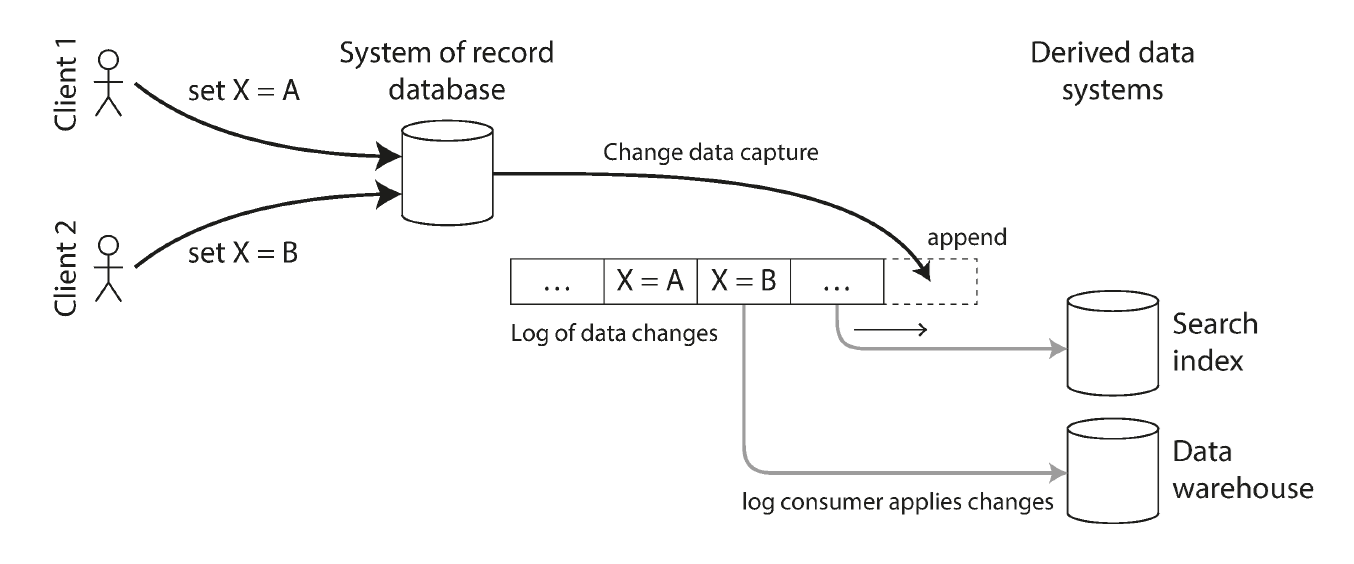
\includegraphics[width=0.8\textwidth]{resources/chapter-2/cdc.png}
    \caption{\textit{CDC Illustration \parencite{dataIntensiveApplications}}}
    \label{fig:cdc-illustration}
\end{figure}

PostgreSQL juga mendukung CDC dengan istilah \textit{logical replication}. Mekanisme ini menggunakan model \textit{publish} dan \textit{subscribe}. PostgreSQL yang mengirimkan \textit{log} bertindak sebagai \textit{publisher}, lalu terdapat \textit{subscriber} lain yang mengonsumsi \textit{log} yang dipublikasikan. \textit{Subscriber} ini bisa berupa replika PostgreSQL lagi atau aplikasi lainnya \parencite{pgLogicalReplication}. PostgreSQL mendukung dua mode operasi untuk replikasi, yaitu replikasi secara \textit{asynchronous} dan \textit{synchronous} \parencite{insideLogicalReplication}. Pada mode \textit{synchronous}, \textit{subscriber} harus merespons terlebih dahulu terhadap perubahan data sebelum PostgreSQL dapat melakukan \textit{commit}.

\begin{figure}[ht]
    \centering
    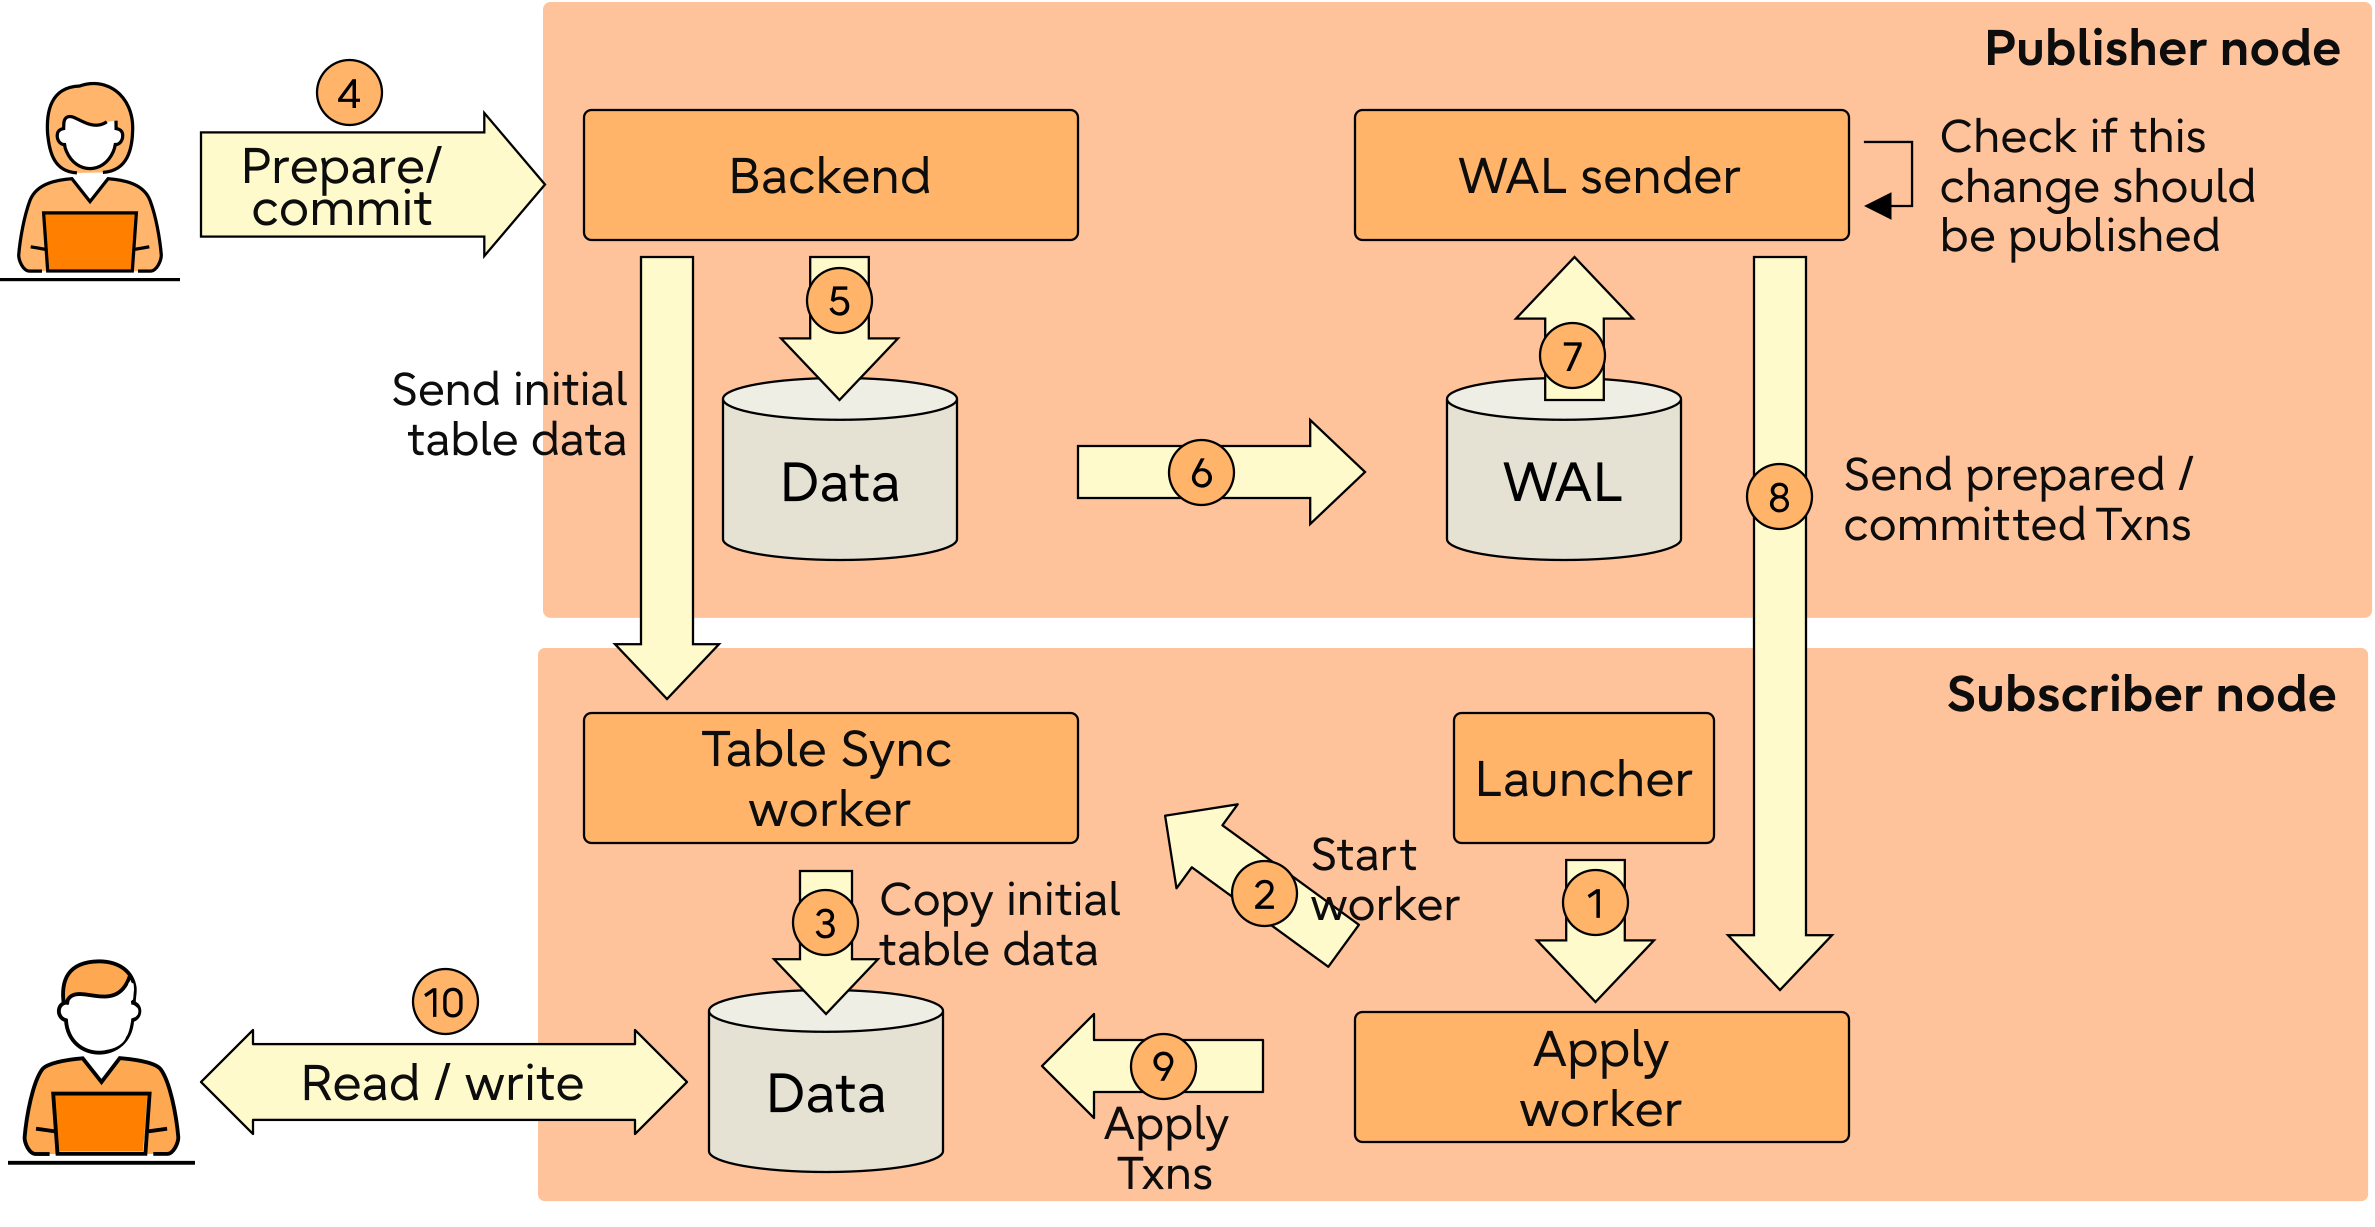
\includegraphics[width=0.8\textwidth]{resources/chapter-2/postgres-logical-replication.png}
    \caption{\textit{Logical Replication Architecture \parencite{insideLogicalReplication}}}
    \label{fig:logical-replication-architecture}
\end{figure}

